\chapter{Agent Micro-ROS}

\section{Installation}

La communication dans ROS2 entre un ordinateur et un microcontrôleur moins puissant est réalisé par un agent Micro-ROS. Cet agent joue le rôle d'intermédiaire, permettant l'intégration de dispositifs à puissance limitée dans un réseau ROS2. Le processus d'installation de ces agents est détaillé sur le site suivant : \url{https://micro-xrce-dds.docs.eprosima.com/en/latest/installation.html}.

Ouvrez un terminal et exécutez les commandes suivantes :

\begin{lstlisting}[style=commandstyle]
git clone https://github.com/eProsima/Micro-XRCE-DDS-Agent.git
cd Micro-XRCE-DDS-Agent
mkdir build && cd build
cmake ..
make
sudo make install
sudo ldconfig /usr/local/lib/
\end{lstlisting}
\underline{Note :} L'opération \textit{make} peut prendre plus d'une heure.

\section{Utilisation}

\noindent Une fois l'installation terminée, il est possible de démarrer un agent avec la commande suivante :

\begin{lstlisting}[style=commandstyle]
MicroXRCEAgent serial --dev /dev/ttyACM0 -b 115200
\end{lstlisting}

\noindent Si l'agent est correctement installé, les lignes suivantes doivent s'afficher dans la console : 
\begin{figure}[H]
    \centering
    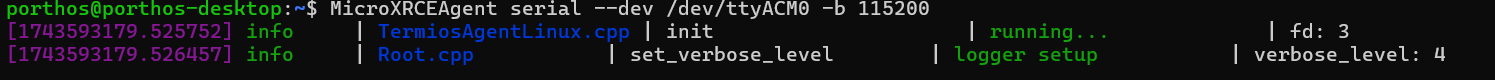
\includegraphics[width=1\textwidth]{Annexes/Mecanum_ROS2/Micro ros agent/pictures/lancement_agent.png}
    \caption{Lancement de l'agent}
\end{figure}

\noindent De plus, si l'OpenCR est correctement programmée (voir partie programmation de l'OpenCR) et que la communication est réussite, d'autres lignes peuvent apparaître :
\begin{figure}[H]
    \centering
    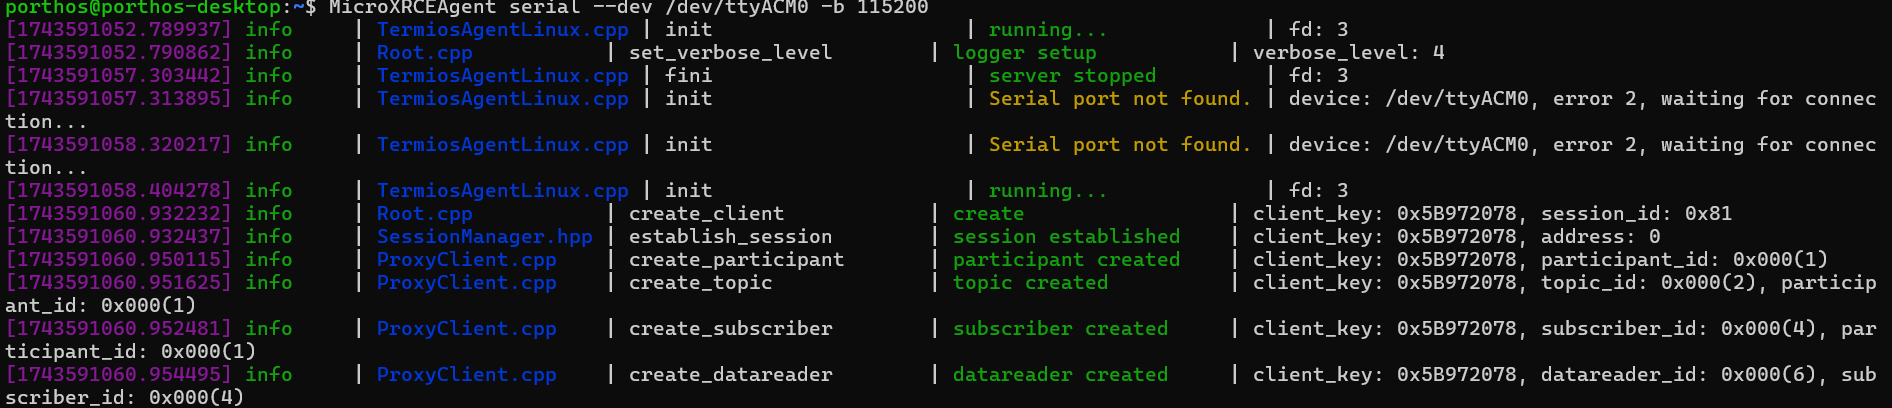
\includegraphics[width=1\textwidth]{Annexes/Mecanum_ROS2/Micro ros agent/pictures/lancement_agent_reussi.png}
    \caption{Lancement de l'agent avec OpenCR}
    \label{pic:agent_reussi}
\end{figure}

\noindent Dans le cas ou l'OpenCR est correctement programmé et que l'Agent s'est lancé, mais que les lignes supplémentaires de la figure \ref{pic:agent_reussi} n'apparaissent pas, cela signifie que la communication entre la Raspberry Pi et l'OpenCR ne s'est pas faite. Dans ce cas, il faut réinitialiser l'OpenCR en appuyant sur le bouton \textit{reset} (voir Figure \ref{pic:reset_button}). 

\begin{figure}[H]
    \centering
    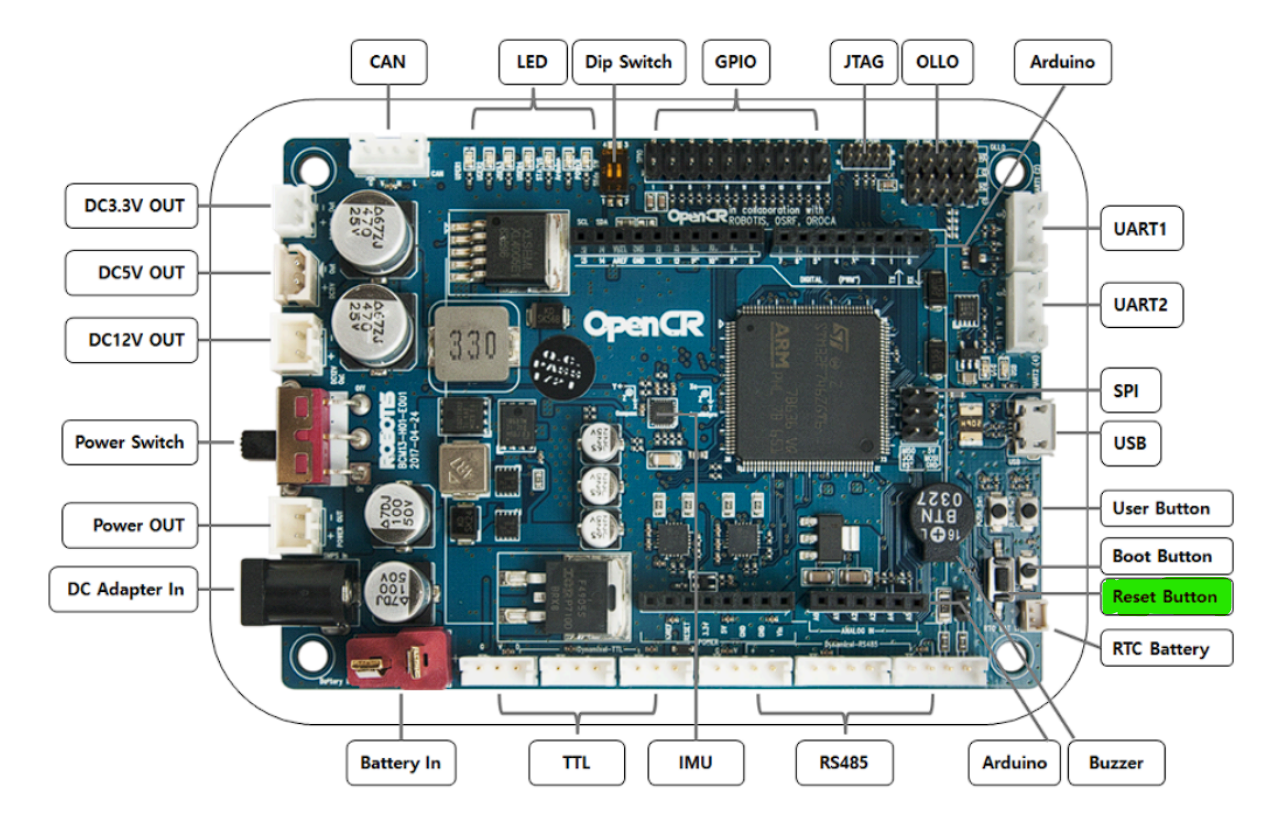
\includegraphics[width=1\textwidth]{Annexes/Mecanum_ROS2/Micro ros agent/pictures/Reset.png}
    \caption{Pinout OpenCR}
    \label{pic:reset_button}
\end{figure}

\noindent Si tout est correctement configuré, les topics auxquels doit avoir accès l'OpenCR seront visibles en utilisant la commande :

\begin{lstlisting}[style=commandstyle]
ros2 topic list
\end{lstlisting}

\section{Utilisation via un service}

Un service sur Ubuntu permet d’exécuter automatiquement une commande au démarrage de la Raspberry Pi. Ici, nous souhaitons lancer automatiquement le Micro-Ros Agent.

\noindent Créer le fichier de service en exécutant la commande suivante :

\begin{lstlisting}[style=commandstyle]
sudo nano /etc/systemd/system/microxrce.service
\end{lstlisting}
\newpage
\noindent Y ajouter le contenu suivant :

\begin{lstlisting}[style=commandstyle]
# /etc/systemd/system/microxrce.service

[Unit]
Description=MicroXRCEAgent
After=network.target

[Service]
ExecStart=/usr/local/bin/MicroXRCEAgent serial --dev /dev/ttyACM0 -b 115200
Restart=always

[Install]
WantedBy=multi-user.target
\end{lstlisting}

\noindent Après avoir créé ou modifié le fichier de service, recharger \textit{systemd} afin de prendre en compte les modifications :

\begin{lstlisting}[style=commandstyle]
sudo systemctl daemon-reload
\end{lstlisting}

\noindent Pour permettre au service de se lancer automatiquement au démarrage du système, exécuter la commande suivante :

\begin{lstlisting}[style=commandstyle]
sudo systemctl enable microxrce.service
\end{lstlisting}

\noindent Pour démarrer immédiatement le service sans attendre le prochain redémarrage du système, exécuter :

\begin{lstlisting}[style=commandstyle]
sudo systemctl start microxrce.service
\end{lstlisting}

\noindent Dans le cas ou la Raspberry Pi est redémarrée, ne pas hésiter à regarder si tous les topics utiles au projet (par exemple, ceux auxquelles souscrit ou publie l'OpenCR) sont visibles via la commande :

\begin{lstlisting}[style=commandstyle]
ros2 topic list
\end{lstlisting}

\noindent S'il ne sont pas visibles, appuyer sur le bouton \textit{reset} de l'OpenCR (voir Figure \ref{pic:reset_button}) pour rédémarrer la communication.

\noindent D'autres commandes utiles pour gérer le service : 

\begin{itemize}
    \item Stopper le service
\end{itemize}

\begin{lstlisting}[style=commandstyle]
sudo systemctl stop microxrce
\end{lstlisting}

\begin{itemize}
    \item Redémarrer le service
\end{itemize}

\begin{lstlisting}[style=commandstyle]
sudo systemctl restart microxrce
\end{lstlisting}



